%%%%%%%%%%%%%%%%%%%%%%%%%%%%%%%%%%%%%%%%%%%%%%%%%%%%%%%%%%%%%%%%%%%%%%%%%%%%%%%
% Definición del tipo de documento.                                           %
% Posibles tipos de papel: a4paper, letterpaper, legalpapper                  %
% Posibles tamaños de letra: 10pt, 11pt, 12pt                                 %
% Posibles clases de documentos: article, report, book, slides                %
%%%%%%%%%%%%%%%%%%%%%%%%%%%%%%%%%%%%%%%%%%%%%%%%%%%%%%%%%%%%%%%%%%%%%%%%%%%%%%%
\documentclass[a4paper,10pt]{article}


%%%%%%%%%%%%%%%%%%%%%%%%%%%%%%%%%%%%%%%%%%%%%%%%%%%%%%%%%%%%%%%%%%%%%%%%%%%%%%%
% Los paquetes permiten ampliar las capacidades de LaTeX.                     %
%%%%%%%%%%%%%%%%%%%%%%%%%%%%%%%%%%%%%%%%%%%%%%%%%%%%%%%%%%%%%%%%%%%%%%%%%%%%%%%

% Paquete para inclusión de gráficos.
\usepackage{graphicx}
\usepackage{float}

% Paquete para definir la codificación del conjunto de caracteres usado
% (latin1 es ISO 8859-1).
\usepackage[utf8]{inputenc}

% Paquete para definir el idioma usado.
\usepackage[spanish]{babel}

% Define una macro para código
\def\code#1{\texttt{#1}}

\begin{document}
% Título principal del documento.
\title{\textbf{Trabajo Practico 1}}

\maketitle

	\begin{table}[h!]
	  \centering
	  \begin{tabular}{ccc}
		\toprule
		Apellido y Nombre & Padrón & Correo electrónico	\\
		\midrule
		Alvarez Avalos, Dylan Gustavo & 98225 & dylanalvarez1995@gmail.com\\
		Gerstner, Facundo Agustin & 96255 & facugerstner\_29@hotmail.com\\
		\bottomrule
	  \end{tabular}
	\end{table}

\date{}
\newpage

% Quita el número en la primer página.
\thispagestyle{empty}


\section{Introducción}
  
   El objetivo del presente trabajo practico es familiarizarse con el conjunto de instrucciones MIPS32 y el concepto de ABI, a través de la implementación de un programa portable que calcula el mínimo común múltiplo y el máximo común divisor entre dos números, utilizando el algoritmo de Euclides para este ultimo. El programa recibe como argumentos dos números naturales e imprime el resultado por stdout o en un archivo si se le especifica.


\section{Implementación}
    El código fuente fue escrito en la maquina host y luego fue enviado para la compilación y ejecución a la maquina guest. Éstas fueron conectadas vía SSH y el pasaje de archivos se llevó a cabo mediante SCP.\\
    Se implementó en C la función \code{main}, que procesa los argumentos de entrada y llama a las funciones \code{mcd} y/o \code{mcm} según corresponda. Estas dos ultimas fueron implementadas en assembler MIPS32. De esta manera se provee soporte especifico para la plataforma principal de desarrollo utilizada en el curso, NetBSD.\\
    La función \code{mcd} calcula el máximo común divisor entre dos números naturales utilizando el algoritmo de Euclides. Al ser dicho algoritmo de naturaleza recursiva, optamos por implementarlo de esa manera, ya que el código es más simple, además de que el stack de la subrutina no es lo suficientemente grande como para ser un problema.\\
    Para la implementación, primero se procedió a implementar las funciones \code{mcm} y \code{mcd} en C (secciones 5.4 y 5.5), para luego realizar un diagrama de stack de ambas funciones, con el objetivo de facilitar la implementación en assember. Finalmente, en base a la implementación en C y a los diagramas, se escribieron dichas funciones. El siguiente diagrama, representa el stack de la funcion mcd:\\
    
    \begin{figure}[H]
        \centering
        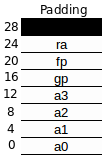
\includegraphics[scale=0.6]{DS_mcd.png}
        \caption{Diagrama de stack de la funcion mcd}
        \label{fig:my_label}
    \end{figure}
    
    La función mcm presenta el mismo diagrama de stack puesto que también es una función no-hoja y guarda la misma cantidad de argumentos.\\

    \subsection{Consideraciones}
    \subsubsection{Proceso de compilación}
    El programa fue compilado con la versión de gcc incluida en el sistema operativo NetBSD, con la siguiente instrucción:\\
    \begin{verbatim}
        root@:~# gcc -Wall -Werror -std=c99 -pedantic -o common
        main.c mcd.S mcm.S
    \end{verbatim}
    Se utilizaron dichas directivas con el objetivo de respetar el estándar 99 de c y evitar warnings. Los archivos assembly poseen la extensión .S con el objetivo de que el código sea procesado por el pre-compilador y asi poder utilizar \#defines y sintaxis de registros (fp en vez de \$30, entre otros), con el objetivo de mejorar la claridad del código.
    
    \subsection{Criterios}
    Existen tres criterios a destacar:\\
    Primero, se tomaron 0 como código de éxito y 1 como código de error.\\
    Segundo, el rango válido para ingresar un numero es de 2 a \code{MAX\_INPUT=1073741823}, que es el máximo valor que permite que \code{mcm(MAX\_INPUT, 2)} compute el resultado correctamente operando con enteros de 32 bits (dado que \code{(MAX\_INPUT + 1) * 2 = 1073741824 * 2 > INT\_MAX}). Consideramos hacer que \code{MAX\_INPUT=46340}, ya que esto garantizaría que todo producto posible quepa en un entero de 32 bits, pero se estarían eliminando muchas posibilidades en nombre de la robustez.\\
    Y tercero, se tomó como salida de errores la estándar (stderr), donde los errores que se pueden imprimir son errores de archivos o de salida del rango válido antes mencionado.\\


\section{Casos de prueba}

    Se realizaron pruebas al programa implementado con distintos valores, con el objetivo de corroborar su correcto funcionamiento. Los casos de pruebas corridos fueron los siguientes:
    \begin{itemize}
        \item ./common 5 10
        \item ./common -d 5 10
        \item ./common -m 5 10\\
        \\El programa funciono de manera correcta, arrojando los valores 5 y 10 para el primer caso, 5 para el segundo, y 10 para el tercero
        \item ./common 256 192
        \item ./common -d 256 192
        \item ./common -m 256 192\\
        \\Nuevamente arrojo los valores correctos, siendo los mismos 64 y 768 para el primer caso, 68 para el segundo y 768 para el tercer caso.
        \item ./common 1073741823 2
        \item ./common -d 1073741823 2
        \item ./common -m 1073741823 2\\
        \\Arrojó los valores correctos en todos los casos.
        \item ./common 1073741824 2
        \item ./common -d 1073741824 2
        \item ./common -m 1073741824 2\\
        \\Advirtió que salimos del rango válido (The number is out of range (2 to 1073741823)).
        \item ./common 1073741823 -12
        \item ./common -d 1073741823 -12
        \item ./common -m 1073741823 -12\\
        \\Advirtió que 1 y 2 no son opciones válidas (por si fuera nuestra intención usar esos caracteres como flags), y que salimos del rango válido (The number is out of range (2 to 1073741823)).\\
        \\Adicionalmente se realizaron las mismas pruebas pero cambiando la salida a un archivo. El programa respondió de manera correcta, creando en cada caso un archivo con los resultados impresos en el mismo. Los comandos ejecutados fueron los siguientes:
        \begin{itemize}
            \item ./common -o results.out 5 10
            \item ./common -o results.out 256 192
            \item ./common -o results.out 1111 1294
        \end{itemize}
    \end{itemize}
    
    A continuacion se presenta un diagrama de stack para el caso de prueba con los valores 256 y 192.\\
    
    \begin{figure}[H]
        \centering
        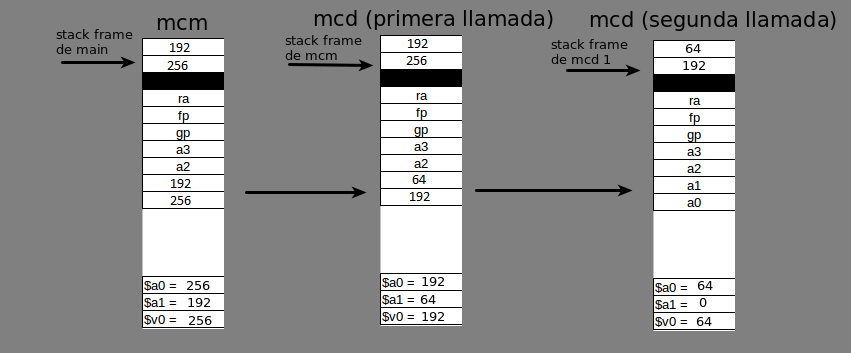
\includegraphics[scale=0.6]{DS_mcm.png}
        \caption{Diagrama de stack de las funciones mcd y mcm al ejecutarce con los parametros 256 y 192}
        \label{fig:my_label}
    \end{figure}
    
    Cuando el registro a1 queda en cero la función termina, quedando en el registro v0 el resultado.\\
    
    
\section{Conclusiones}
    La presencia de la ABI hace que este simple programa recursivo ocupe mucho más espacio en memoria que el realmente necesario, si bien otorga órden en el código y un necesario consenso para la comunicación entre distintos binarios.\\
    Luego de implementada nuestra versión del código assembly, vimos el código generado por gcc y nuestra versión C de \code{mcd}, para las distintas configuraciones de optimización, y resulta que existen varias diferencias. Dentro de las principales diferencias nos encontramos con que, gcc lo resuelve de manera iterativa, lo que lleva a una mayor complejidad en el código. Además utiliza mas espacio de stack ya que guarda y utiliza el registro s0. Confrontando ambas implementaciones en assembly, medimos el tiempo de compilación para ambos casos anteponiendo al comando de compilación el comando time, obteniendo un valor de 2.234 segundos con los assembler de gcc y 2.164 segundos con nuestro código assembler. Sin embargo en la ejecución, el binario de gcc fue el mas rápido, con 0.035 segundos frente a 0.051 segundos para la prueba con los valores 256 y 192. En el resto de las pruebas (con distintos valores) la diferencia en los tiempos fue aproximadamente la misma.\\
    La diferencia no es muy grande, pero el programa implementado es sencillo, frente a problemas mas complejos, es necesario que el código assembler sea lo mas optimizado posible para generar un binario rápido. Y si bien nuestro assembler compilo mas rápido, lo importante es la velocidad de ejecución, ya que, un programa se compila una vez y se ejecuta varias veces.\\
    Además comparamos el tiempo de compilación y ejecución de nuestra aplicación compilada con el código assembly y con C. Por un lado, la compilación con los assembler fue notablemente mas rápida, con 2.195 segundos frente a 3.902 segundos que tardo la compilación con los archivos C. Esto era esperado, ya que gcc debía generar el assembler de las funciones en C y después generar el ejecutable. En cuanto a la ejecución, los tiempos fueron casi iguales, con una diferencia de 0.004 segundos.\\
    Si bien programar en assembler puede ser complejo, es necesario en situaciones donde se quiera tener un control absoluto sobre la velocidad o tamaño de un programa. Estas situaciones son las que se encuentran, por ejemplo, a la hora de programar para una computadora embebida.

\section{Apéndice}
A continuación se presenta el código escrito para el presente trabajo.\\

\subsection{main.c}
  \begin{verbatim}

#include <stdio.h>
#include <stdbool.h>
#include <string.h>
#include <stdlib.h>
#include <getopt.h>
#include <errno.h>
#include <limits.h>

#define SUCCESS 0
#define ERROR 1
#define VERSION 1.0
#define MIN_USER_INPUT 2
#define MAX_USER_INPUT 1073741823

extern int mcd(int, int);

extern int mcm(int, int);

void print_info() {
  printf("%s\n%s\n%s\n%s\n",
         "Usage:",
         "  common -h",
         "  common -V",
         "  common [options] M N");
  printf("%s\n%s\n%s\n%s\n%s\n%s\n",
         "Options:",
         "  -h, --help     Prints usage information",
         "  -V, --version  Prints version information",
         "  -o, --output   Path to output file",
         "  -d, --divisor  Just the divisor",
         "  -m, --multiple Just the multiple");
  printf("%s\n%s\n",
         "Examples:",
         "  common -o - 256 192");
}

void print_version() {
  printf("%s%.2f\n", "Version: ", VERSION);
}

void print_out_of_range_error() {
  fprintf(stderr, "The number is out of range (%d to %d)\n", MIN_USER_INPUT,
          MAX_USER_INPUT);
}

int main(int argc, char **argv) {
  int argument;
  FILE *output = NULL;
  char *lastChar;
  bool returnMultiple = true;
  bool returnDivisor = true;
  int argumentsRecievedByGetopt = 0;

  static struct option options[] =
      {
          {"help",     no_argument,       NULL, 'h'},
          {"version",  no_argument,       NULL, 'V'},
          {"output",   required_argument, NULL, 'o'},
          {"divisor",  no_argument,       NULL, 'd'},
          {"multiple", no_argument,       NULL, 'm'},
          {NULL,       no_argument,       NULL, 0}
      };

  while ((argument = getopt_long(argc, argv, "hVo:dm", options, NULL)) != -1) {
    switch (argument) {
      case 'd':
        argumentsRecievedByGetopt++;
        returnMultiple = false;
        break;
      case 'm':
        argumentsRecievedByGetopt++;
        returnDivisor = false;
        break;
      case 'h':
        print_info();
        return SUCCESS;
      case 'V':
        print_version();
        return SUCCESS;
      case 'o':
        argumentsRecievedByGetopt += 2;
        if (strcmp(optarg, "-") != 0) {
          output = fopen(optarg, "wb");
          if (!output) {
            fprintf(stderr,
                    "The file '%s' could not be created/opened\n",
                    optarg);
            return ERROR;
          }
        }
      default:
        break;
    }
  }
  long numbers[2];
  bool strtolError;
  bool resultWillBeValid;
  for (int i = 0; i < 2; i++) {
    numbers[i] = strtol(argv[argumentsRecievedByGetopt + 1 + i], &lastChar, 10);
    strtolError = errno == ERANGE &&
                  (numbers[i] == LONG_MIN || numbers[i] == LONG_MAX);
    resultWillBeValid =
        numbers[i] >= MIN_USER_INPUT && numbers[i] <= MAX_USER_INPUT;
    if (strtolError || (!resultWillBeValid)) {
      print_out_of_range_error();
      return ERROR;
    }
  }

  if (returnDivisor) {
    fprintf(output ? output : stdout, "%d\n",
            mcd((int) numbers[0], (int) numbers[1]));
  }

  if (returnMultiple) {
    fprintf(output ? output : stdout, "%d\n",
            mcm((int) numbers[0], (int) numbers[1]));
  }

  if (output) { fclose(output); }
  return SUCCESS;
}

  \end{verbatim}
 
 \subsection{mcd.S}
 \begin{verbatim}
 #include <mips/regdef.h>

#define fp $30
#define gp $28

	.text
	.globl mcd
	.ent mcd
mcd:
	subu	sp,sp,32	# Saved Register Area
	sw		ra,24(sp)
	sw 		fp,20(sp)	
	sw 		gp,16(sp)	
	move 	fp,sp

	sw 		a0,32(sp)		# Argument Building Area	
	sw		a1,36(sp)
	sw		a2,40(sp)
	sw		a3,44(sp)

	lw		v0,32(sp)
	lw		v1,36(sp)

	beq		v1,0,fin		# Si a1 es cero termino
	
	move 	a0,v1		# seteo de argumentos para la llamada recursiva
	rem 	a1,v0,v1
	jal 	mcd

fin:
	lw 		ra,24(sp)
	lw 		fp,20(sp)
	addu 	sp,sp,32
	j 		ra
	.end mcd
 \end{verbatim}
  
  \subsection{mcm.S}
  \begin{verbatim}
#include <mips/regdef.h>

#define fp $30
#define gp $28

	.text
	.globl mcm
	.extern mcd
	.ent mcm
mcm:
	subu	sp,sp,32	# Saved Register Area
	sw		ra,24(sp)
	sw 		fp,20(sp)	# el regsitro 30 es fp
	sw 		gp,16(sp)	# el registro 28 es gp
	move 	fp,sp

	sw 		a0,32(sp)	# Argument Building Area	
	sw		a1,36(sp)
	sw		a2,40(sp)
	sw		a3,44(sp)

	jal 	mcd

	lw		a0,32(sp)
	lw		a1,36(sp)
	mul		a0,a0,a1
	divu	v0,a0,v0			

	lw 		ra,24(sp)	# fin
	lw 		fp,20(sp)
	addu 	sp,sp,32
	j 		ra
	.end mcm
  \end{verbatim}
  
  \subsection{mcd.c}
  \begin{verbatim}
int mcd(int a, int b){
	   if (a == 0){
	       return a;
	   } else {
	       return mcd(a, a % b);
	   }
}
    \end{verbatim}
    
   \subsection{mcm.c}
   \begin{verbatim}
extern int mcd(int, int);

int mcm(int a, int b){
	    return ( (a * b) / mcd(a, b) );
}

   \end{verbatim}

\end{document}
